\documentclass[11pt,a4paper]{article}
\usepackage[utf8]{inputenc}
\usepackage[T1]{fontenc}
\usepackage[english]{babel}
\usepackage[margin=2.4cm]{geometry}
\usepackage{amsmath,amssymb}
\usepackage{booktabs}
\usepackage{longtable}
\usepackage{graphicx}
\graphicspath{{images/}}
\usepackage{xcolor}
\usepackage[colorlinks=true,linkcolor=blue!60!black,urlcolor=blue!60!black]{hyperref}

\newcommand{\dir}{\widehat{\Theta}}
\newcommand{\cruise}{\mathrm{c}}
\newcommand{\brake}{\mathrm{b}}
\newcommand{\obj}{\mathrm{obj}}
\newcommand{\code}[1]{\texttt{#1}}

\title{\textbf{A simulator for bidirectional ant traffic}\\[4pt]
       \large Model, parameters and methods}
\author{Technical companion to the \code{simulateur/} directory}
\date{\today}

\begin{document}
\maketitle

\begin{abstract}
\noindent This document records the model as actually implemented in the
\code{simulateur/} directory, the provenance of each of its parameters, and the
protocols used to measure the observables. It follows on from the hand-off
report \emph{An individual-based model for bidirectional ant traffic on a
narrow bridge}, whose microscopic model and unit conventions it keeps; it
departs from it on five points, all listed in \S\ref{sec:gaps} together with
the measurement that motivates each. The guiding principle is that every number
should be traceable: for each parameter we state whether it is \emph{measured}
on the experimental trajectories, \emph{calibrated} against a macroscopic
observable, or \emph{inherited} from the reference model without any new
constraint.
\end{abstract}

\tableofcontents
\bigskip

%======================================================================
\section{Scope}

The simulator lives in \code{simulateur/}, independently of the reference code,
which it does not modify. It implements the same microscopic model --- decoupled
radial/angular dynamics, interaction repertoire, thigmotaxis --- with an
architecture rebuilt to make parameter sweeps and reproducible measurements
possible.

Internal units are those of the hand-off report: \textbf{1 length unit = 1 mm},
\textbf{1 time unit = 1 s}, ant of radius $R = 1$. Conversions to the units of
Poissonnier et al.\ (2019) are
$k\,[\mathrm{cm^{-2}}] = \rho\,[\mathrm{mm^{-2}}]\times 100$ and
$q\,[\mathrm{cm^{-1}s^{-1}}] = 10\,\rho\,U$.

%======================================================================
\section{The model}

\subsection{Variables and dynamics}

Each agent $i$ carries a position $X_i\in\mathbb R^2$, a \emph{scalar} speed
$u_i\geq0$, a heading $\theta_i$ and a fixed group
$\mathrm g_i\in\{-1,+1\}$ ($+1$ towards the food, $-1$ towards the nest). The
vector velocity is $V_i = u_i\dir_i$ with $\dir_i = (\cos\theta_i,\sin\theta_i)$.
Positions evolve through $\dot X_i = u_i \dir_i$, and the two velocity
components obey two separate relaxation equations:
\begin{align}
\frac{\mathrm du_i}{\mathrm dt}
  &= (\nu_\cruise+\nu_\brake)\Big(\tfrac{\nu_\cruise}{\nu_\cruise+\nu_\brake}\,\xi_i-u_i\Big),
  \label{eq:radial}\\[2pt]
\frac{\mathrm d\theta_i}{\mathrm dt} &= \lambda\,\sin(\omega_i-\theta_i),
  \qquad \omega_i=\arg F_i .
  \label{eq:angular}
\end{align}

Equation~\eqref{eq:radial} is the core of the model: braking enters as a
\emph{rate} of relaxation, not as a subtracted force. Under a mono-kinetic
closure where $\nu_\brake \simeq \bar\beta k$, the equilibrium speed is
$U(k)=\xi\nu_\cruise/(\nu_\cruise+\bar\beta k)$ and the flow $q=kU$
\emph{saturates} instead of collapsing --- this is the mechanistic origin of the
plateau.

\subsection{Angular dynamics: three modes}\label{sec:angular}

Written as it stands, the hand-off report's equation ($\lambda = |F_i|$) makes
the norm of the field play two roles at once: it sets the target direction
\emph{and} the rate at which the agent turns towards it. A strong repulsion term
therefore makes the turn nearly instantaneous, which forces a cap on
$|\dot\theta|$ --- a cap that then mixes heterogeneous scales. The simulator
exposes three choices, selected by \code{angular\_mode}:

\begin{center}
\begin{tabular}{@{}lll@{}}
\toprule
\code{angular\_mode} & $\lambda$ & Comment \\
\midrule
\code{field\_norm} (default) & $|F_i|$, capped at \code{lambda\_max} & the hand-off report's equation \\
\code{fixed} & \code{lambda\_theta} & the $c_\bullet$ then set only a relative priority \\
\code{saturating} & $\lambda_{\max}|F|/(|F|+F_{\rm ref})$ & graded response, bounded by construction \\
\bottomrule
\end{tabular}
\end{center}

The \code{fixed} mode is the clean extension of the Persistent Turning Walker
and makes \code{lambda\_theta} directly calibrable against the measured
distribution of angular velocities; it is the recommended variant for the
calibration phase. The default remains \code{field\_norm} so that the simulator
reproduces the reference model.

\emph{A strict priority logic was deliberately not adopted}: it would introduce
discontinuities in the drift field, breaking the Lipschitz-kernel assumption of
the mean-field limit, and with it the bridge towards the macroscopic
description.

\subsection{Interaction kernels}

Each term factorises into (strength) $\times$ (distance profile) $\times$
(angular profile) $\times$ (direction), with $\rho=|X_j-X_i|$,
$\sigma_{ij}=(X_j-X_i)/\rho$, and the cone factor
$A_\varepsilon(\alpha)=\big[(\varepsilon-(1-\cos\alpha))/\varepsilon\big]_+$.
Only two distance profiles are used: a \emph{singular} one $(\ell-\rho)/\rho$
for the contact behaviours, and a \emph{ramp}
$(\rho-\ell_{\min})/(\ell_{\max}-\ell_{\min})$ for the attraction-at-distance
behaviours.

\begin{center}
\begin{tabular}{@{}llll@{}}
\toprule
Term & Groups & Support & Direction \\
\midrule
braking ($\to\nu_\brake$) & all & $\rho\leq\ell_\brake$, frontal cone & --- (radial) \\
avoidance & opposite & $\rho\leq\ell_{\rm avoid}$, frontal cone & $\pm\sigma^\perp$ (disengaging) \\
antennation & opposite & $\ell_{\rm avoid}<\rho\leq\ell_{\rm comm}$, frontal cone & $+\sigma$ \\
lateral repulsion & same & $\rho\leq\ell'_{\rm avoid}$, lateral & $-\sigma$ \\
overtaking & same & $\rho\leq\ell_{\rm over}$, frontal cone, $u_j\leq\alpha\xi_i$ & $\sigma^\perp$ towards goal \\
following & same & $\ell_f<\rho\leq\ell'_f$, frontal cone & $+\sigma$ \\
objective & --- & --- & $k_\obj\,(\mathrm g,0)$ \\
wall & --- & $\ell_{\min}<d\leq\ell_{\max}$ & $\sigma_{\rm wall}$ \\
\bottomrule
\end{tabular}
\end{center}

Every term can be switched on or off independently (\code{use\_brake},
\code{use\_comm}, \ldots), which makes ablations immediate.

\subsection{Thigmotaxis: three laws}\label{sec:wall}

This is where the simulator departs most from the reference model, and the
decision rests on a measurement. The hand-off report's law
(\code{wall\_law = tangential}) weights the attraction by the \emph{tangential}
component of the heading: it is therefore \emph{maximal when the agent is
already walking along the wall}. Three measurements show that this makes the
wall an absorbing state:

\begin{itemize}\itemsep2pt
\item an \textbf{isolated} agent, with no neighbour at all, starting from the
      centre, spends \textbf{98\,\%} of its time within 1 mm of a wall;
\item the wall fraction \textbf{does not settle}: 24\,\% at 2~s, 38\,\% at
      10~s, 40--46\,\% beyond 40~s (with no thigmotaxis: 3--6\,\%);
\item it depends on bridge width at equal linear density:
      47 / 36 / 23\,\% for $W=5/10/20$ mm.
\end{itemize}

Mechanically: the force is \emph{never} repulsive (zero if the agent is moving
away, attractive otherwise), its radial profile \emph{increases} with distance
(zero at $\ell_{\min}$, maximal at $\ell_{\max}=4$), and on a 10 mm bridge the
active band covers 70\,\% of the width with its maximum immediately next to the
centreline, of magnitude $10 = k_\obj$. The centreline is therefore an unstable
separatrix, and the wall band a well whose restoring force \emph{grows} with the
escape distance.

The simulator adds two laws. \code{outward\_damping} only holds back an agent
that is moving away; it fixes the weighting but remains one-sided and never
initiates wall-following (it simply freezes $y$). \code{standoff} (default)
restores the agent towards a target distance $\ell_{\rm standoff}$,
\textbf{repulsive below it}, attractive above:
\[
F_{\rm wall} = c_{\rm wall}\,w(d)\,\sigma_{\rm wall},
\qquad
w(d)=\begin{cases}\frac{d-d^\star}{\ell_{\max}-d^\star} & d\geq d^\star,\\[2pt]
\frac{d-d^\star}{d^\star} & d<d^\star.\end{cases}
\]
What it produces, \emph{measured} at the default parameters, is a wall
\textbf{preference}, not an equilibrium: an isolated agent still wanders across
the full width of the channel (distance to the wall from 0.5 to 5.0 mm, mean
1.9 on a half-width of 5), but it is never crushed against the edge (3\,\% of
agents within 0.5 mm, against 30\,\% for \code{tangential}). That is the real
gain of this law; the target distance is a soft attractor, not a fixed point.

\medskip
\noindent Comparison on three criteria (single agent, head-on pair against the wall,
crowd; \code{scripts/diagnose\_wall.py}):

\begin{center}
\begin{tabular}{@{}lcccc@{}}
\toprule
\code{wall\_law} & single agent: final $d$ & segregation & \% crushed & speed \\
\midrule
\code{tangential}, $c_{\rm wall}=10$ & 0.47 (crushed) & 0.29 & 0.30 & 8.63 \\
\code{outward\_damping} & 1.00, no capture & 0.23 & 0.15 & 8.50 \\
\code{standoff}, $c_{\rm wall}=10$ & 1.00 & \textbf{0.92} (lanes!) & 0.12 & 13.42 \\
\textbf{\code{standoff}, $c_{\rm wall}=2$} & \textbf{1.00} & \textbf{0.32} & \textbf{0.11} & 9.61 \\
\bottomrule
\end{tabular}
\end{center}

$c_{\rm wall}=10$ had been calibrated for the \code{tangential} law, where the
force is strongly attenuated; the \code{standoff} law applies the full
$c_{\rm wall}$ to the offset from the target distance and therefore needs
recalibrating. At $c_{\rm wall}=2$ all three criteria are met without degrading
the mixing.

\emph{Known limitation, shared by all three laws}: in an exactly symmetric
configuration (two agents at the same ordinate, same tie-breaking sign) the
avoidance steering cancels and the pair deadlocks. This is a measure-zero case
--- a 0.2 mm offset is enough for all three laws to cross cleanly --- and it is
what the report's \emph{wall-escape} term addressed; that term is kept as an
option (\code{use\_wall\_escape}, disabled).

\subsection{Boundary conditions}

\textbf{Side walls.} \code{specular} (default) reverses the normal component of
the heading, \code{slide} removes it. Both enforce zero normal flux; the report
adopts specular reflection, which avoids the wall-sticking that a sliding
condition induces at high density.

\textbf{Bridge ends.} \code{torus} (default): $x$ is periodic and the ordinate
is \textbf{redrawn at random on re-entry}. On a torus of finite length an agent
passes the same place indefinitely; keeping its ordinate lets a transverse
structure freeze in. \code{torus\_keep\_y} keeps $y$ (continuous trajectory),
\code{inflow} reinjects the departing agent at its group's entrance. In all
cases vision remains blocked at the ends (semi-periodicity).

\emph{The remixing has a measured effect on one observable}: it destroys lanes
by construction and therefore \emph{underestimates} the effect of antennation
on mixing. At $N=150$ the segregation excess without antennation is $+0.25$
under \code{torus} against $+0.63$ under \code{torus\_keep\_y}. For that
observable specifically, measurements should be made with
\code{torus\_keep\_y}.

%======================================================================
\section{Parameters}\label{sec:params}

Provenance: \textbf{M} = measured on the experimental trajectories,
\textbf{C} = calibrated against a macroscopic observable, \textbf{I} = inherited
from the reference model with no new constraint, \textbf{D} = modelling
decision.

\begin{center}
\small
\begin{longtable}{@{}llcl@{}}
\toprule
Group & Parameter & Default & Provenance \\
\midrule
\endhead
Geometry & \code{length}, \code{height} & 100, 10 & I (experimental bridge) \\
 & \code{radius} & 1.0 & M -- measured body $3.2\times1.8$ mm, equiv.\ radius 1.2 \\
Perception & \code{angle\_vision}, \code{l\_vision} & $\pi$, 8 & I \\
Radial & \code{nu\_cruise} & 20 & M -- see \S\ref{sec:nu} \\
 & \code{xi\_cruise} & \textbf{14} & M/C -- compromise, see \S\ref{sec:xi} \\
 & \code{xi\_spread} & 0.2 & D -- capped by decision \\
 & \code{nu\_wall\_stop} & $10^{10}$ & D -- radial half of the no-flux condition \\
Angular & \code{angular\_mode} & \code{field\_norm} & I -- see \S\ref{sec:angular} \\
 & \code{k\_obj} & 10 & I \\
 & \code{lambda\_theta}, \code{lambda\_max} & 10, 50 & I \\
 & \code{sigma\_theta} & 0.3 & D -- symmetry breaker, absent from the reference model \\
Braking & \code{l\_brake} & 3.0 & I -- the data suggest $\sim5$ \\
 & \code{eps\_brake}, \code{alpha\_brake} & 0.7, 4 & I \\
 & \code{c\_brake} & 300 & M -- measured $\bar\beta$ 196 vs 175 in the model \\
Avoidance & \code{l\_avoid\_steer}, \code{eps}, \code{c} & 2.3, 0.7, 50 & I \\
Repulsion & \code{l\_repulse}, \code{eps}, \code{c} & 1.5, 2.0, 40 & I \\
Antennation & \code{l\_comm\_min}, \code{l\_comm} & 2.3, 5.0 & I \\
 & \code{eps\_comm}, \code{c\_comm} & 1.0, 12 & C -- 20 clogs over long runs \\
Overtaking & \code{l}, \code{eps}, \code{c}, \code{alpha} & 4, 0.7, 15, 10 & I \\
Following & \code{l1}, \code{l2}, \code{eps}, \code{c} & 3, 8, 0.7, 30 & I \\
Wall & \code{wall\_law} & \code{standoff} & M -- see \S\ref{sec:wall} \\
 & \code{c\_wall} & 2.0 & C -- recalibrated for the \code{standoff} law \\
 & \code{l\_wall\_standoff}, \code{c\_wall\_damping} & 1.0, 1.0 & D -- data suggest 2.5--4 mm \\
 & \code{l\_wall\_min}, \code{l\_wall\_max} & 0.5, 4.0 & I \\
Boundaries & \code{wall\_mode}, \code{x\_mode} & \code{specular}, \code{torus} & I / D \\
Simulation & \code{dt}, \code{record\_fps} & 0.01, 20 & D \\
\bottomrule
\end{longtable}
\end{center}

\subsection{Cruising speed}\label{sec:xi}

Three observables give three incompatible values:

\begin{center}
\begin{tabular}{@{}lc@{}}
\toprule
What one wants to match & required $\xi$ \\
\midrule
the slope of the diagram measured on the trajectories & $\sim11$ mm/s \\
the free-flow speed measured on the trajectories & 12.5--13 mm/s \\
the published plateau $q_j=10$ & $\sim15$ mm/s \\
\bottomrule
\end{tabular}
\end{center}

They cannot be satisfied together as long as $\xi$ and $\bar\beta$ jointly set
both the slope and the plateau --- and the trajectory data \textbf{do not
arbitrate}, since they stop at $k=4.4$, well before the plateau.
$\xi = 14$ is the compromise adopted: the plateau stays matched (10.20 against
10.0) and the discrepancy on the rise falls to $+9$--$+30$\,\%.

The best measurement of the free-flow speed is not ``the speed of isolated
ants'' (rare at these densities, and the criterion also selects stopped ants)
but the \textbf{plateau of speed as a function of the distance to the neighbour
ahead}:

\begin{center}
\begin{tabular}{@{}lccccccc@{}}
\toprule
distance to the frontal neighbour (mm) & 1.25 & 2.25 & 3.25 & 4.25 & 5.25 & 6.25 & $>8$ \\
mean speed (mm/s) & 5.35 & 7.83 & 11.30 & 12.85 & 13.20 & 12.71 & $\sim$12.2 \\
\bottomrule
\end{tabular}
\end{center}

This profile also gives the braking range: the drop-off begins around
\textbf{5 mm}, not 3. Lengths having been frozen by decision, the discrepancy
is recorded but not corrected.

\subsection{Speed relaxation rate}\label{sec:nu}

The correlation time of speed measured along the tracks is 0.227 s, which
\emph{seems} to impose $\nu_\cruise\approx4.4$. This is an over-interpretation:
that time is not $1/\nu_\cruise$, it is dominated by braking switching on and
off as neighbours pass. Measured \emph{with the same estimator on the
simulation}:

\begin{center}
\begin{tabular}{@{}lccc@{}}
\toprule
 & data & $\nu_\cruise=20$ & $\nu_\cruise=4.4$ \\
\midrule
correlation time (s) & 0.227 & \textbf{0.268} & 0.422 \\
\bottomrule
\end{tabular}
\end{center}

$\nu_\cruise = 20$ is therefore the value \emph{closest to the data}; lowering
it moves away. Confirmed independently on the fundamental diagram: at constant
$\nu_\cruise/c_\brake$ ratio, varying $\nu_\cruise$ by a factor 4.5 changes
neither $k_c$ (17.6 $\to$ 17.9) nor $q_j$ (10.5 $\to$ 10.1). The diagram only
sees the ratio; constraining $\nu_\cruise$ will require a dynamical observable.

%======================================================================
\section{Numerical methods}

\textbf{Integration.} Splitting scheme, with both relaxations solved
\emph{exactly} over the step at frozen field:
$u \leftarrow u\,\mathrm e^{-r\Delta t} + u^\star(1-\mathrm e^{-r\Delta t})$
with $r=\nu_\cruise+\nu_\brake$, and
$\tan\frac{\theta-\omega}{2}\leftarrow\tan\frac{\theta-\omega}{2}\,\mathrm e^{-\lambda\Delta t}$.
Both are unconditionally stable and free of overshoot; $u\geq0$ is preserved
exactly (a convex combination of positive quantities). Positions are then
advected. The update is \emph{synchronous}: everything is read from the current
state and written to the next.

\textbf{Neighbourhoods.} Cell list of mesh $\ell_{\rm vision}$, amortised
$O(N)$ cost, equivalent to the $O(N^2)$ sweep --- verified neighbour by
neighbour, sorted indices included. The walls of the rectangle are handled
analytically (the reference code scanned 250 wall points per agent per step to
find the nearest one, which is $\min(y, H-y)$), and visual occlusion by the wall
is exact by convexity. No allocation inside the per-agent loop.

\textbf{Parameters and compilation.} No \code{@njit} function reads a parameter
as a global variable: everything travels through a \code{NamedTuple} passed as
an argument, and the discrete choices (geometry, angular mode, boundary
condition) are integers branched inside the functions. Numba compiles once; any
other instance then passes without recompilation, which is what makes sweeps
possible.

\textbf{Reproducibility.} All randomness comes from a \emph{single}
\code{np.random.default\_rng(seed)}. The reference code drew random numbers
\emph{inside} the compiled functions; but in nopython mode Numba holds its own
random state, distinct from NumPy's, which forced two generators to be seeded.
The problem was removed rather than managed: degenerate direction tie-breaks use
a sign drawn once per agent, and the noise and reinjection draws are
pre-generated in blocks and passed to the kernel. A test automatically checks
that no \code{np.random} call survives in compiled code. Draws are consumed at
every substep whether or not the noise is active, so the random sequence does
not depend on the model options: \emph{ablations are comparable at equal seed}.

\textbf{Storage.} One run = one \code{config.json} (all parameters, the seed,
the code version) and one \code{trajectories.npz} (compressed float32). The JSON
alone suffices to replay the run identically, which
\code{scripts/replay.py} verifies bit for bit.

%======================================================================
\section{Measurement methods}

\subsection{Fundamental diagram}

Three flow estimators, measured on the \emph{same} runs:
(1) crossings of the central line with the density read in a central
1 cm$^2$ window --- the eLife protocol, and the noisiest;
(2) the same, averaged over 7 cross-sections; (3) whole domain, where $k$ is
exact and $q=\langle\sum|v_x|\rangle/(LW)$. In a stationary regime the mean flow
is the same at every cross-section, so averaging cuts the variance without
introducing bias. The three agree.

\emph{Caution with estimator (1) at high density}: it measures a \emph{local}
density, which legitimately exceeds the global one when a cluster occupies the
window (up to $k=39$ for a global density of 28).

\textbf{Two-phase fit.} Phase 1: mono-kinetic closure
$q=\xi\nu_\cruise k/(\nu_\cruise+\bar\beta k)$ on the low and mid densities.
Phase 2: constant plateau on the high densities \emph{only}. The split is chosen
to maximise the overall $R^2$, and $k_c$ is the abscissa where the two branches
meet.

\textbf{Error bars.} Standard deviation across seeds (the standard error is also
in the CSV). They are small because each point is \emph{already} a time average
over $\sim$24 s of stationary regime, i.e.\ $\sim$480 frames: the instantaneous
fluctuation is averaged out within a run, and all that remains between seeds is
the variability of the initial condition.

\subsection{Antennal contacts}

A pair $(i,j)$ is \emph{in contact} at a given frame if: the groups are
opposite; $\rho\leq d_{\rm contact}=2.5$ mm (the body is $2R=2$ mm, so the
threshold places contact a quarter of a diameter beyond it, representing
antennae touching); and \textbf{each} sees the other within a frontal cone of
$\pm60^\circ$ --- the condition is mutual, so an ant being overtaken from behind
is not an antennal contact.

An \emph{episode} starts at the first frame where the condition becomes true and
ends at the first frame where it becomes false. Resolution: 0.05 s; there is no
hysteresis, so a pair flickering around the threshold is counted several times
--- that is the main limitation.

$C$ is the number of contacts experienced during a \emph{transit} of a central
20 mm section: a continuous stay, with entry \emph{and} exit observed, and no
periodic wrap in between.

\textbf{What depends on conventions.} The \emph{linearity} of $C$ in $k$ is
robust (all conventions, all velocity parameter sets, $R^2\geq0.98$ up to
$k\approx20$): that is what is a property of the model. The \emph{value} of the
slope varies from 0.58 to 0.95 depending on the antennal range adopted (2.2 to
3.5 mm). Agreement at 0.61 therefore constrains the convention as much as it
validates the model; a proper calibration would measure $d_{\rm contact}$ on the
trajectories before comparing slopes.

Beyond $k=20$ the fit stops: the flow has split into clusters, complete transits
become long and rare, and the count becomes noisy ($R^2$ drops to 0.93).

\subsection{Transverse mixing}

The raw index is the occupancy-weighted mean of $|n_+-n_-|/(n_++n_-)$ over 8
horizontal strips. \textbf{It is not zero for a perfectly mixed flow}: with $n$
agents per strip and randomly assigned groups it averages $\sqrt{2/\pi n}$, i.e.
0.29 for 7 agents and 0.14 for 30. It therefore decreases mechanically as
density rises, without any additional mixing taking place --- a trap we fell
into before correcting it.

The baseline is therefore \emph{measured} rather than assumed: at each frame the
group labels are reshuffled at random among the agents present (\emph{positions
are unchanged}) and the index is recomputed. This is the exact null ``observed
positions, groups independent of position''. Only the \textbf{excess} (raw minus
baseline) is interpretable.

\subsection{Space--time diagram}

Local density per $x$-slice and per frame. At $k=6$: diagonal streaks in both
directions, no persistent structure. At $k=25$: bright, persistent vertical
bands --- near-stationary clusters lasting tens of seconds alongside free-flowing
regions --- the phase separation that explains the plateau.

\subsection{Comparison with the published measurements}\label{sec:elife}

Two points of comparison are available, and they must be distinguished.

\textbf{The} \emph{two-phase} \textbf{fit} of the article (linear up to
$k_j=8$, then constant) is the one the hand-off report compared itself to. It is
only one of four fits the article overlays on its data (two-phase, Underwood,
Pipes--Munjal, Greenshields), and ``$k_j=8$'' is a parameter of it, not a
measurement.

\textbf{The published points} (figure 4 of the article, panels A and B) are the
measurements. They were read off by hand and stored in
\code{donnees\_publiees/elife2019\_figure4.csv}; the accuracy is that of a
graphical reading ($\sim$0.05 cm/s, $\sim$0.2 ant/cm/s). These are what one
should compare against, and they say two things the fit conceals:

\begin{itemize}\itemsep2pt
\item \textbf{the cloud has no knee}: $q(k)$ starts bending at $k\approx3$ and
      saturates gradually towards $k\approx12$--14. The shape is that of a
      smooth saturating law, not a broken line --- and that is precisely the
      shape the model produces;
\item \textbf{speed decreases continuously} from $v\approx17.5$ mm/s as
      $k\to0$ down to $\sim$7.5 mm/s at $k=14$, with no intermediate plateau or
      bump.
\end{itemize}

\subsection{Fundamental diagram \emph{of the data}}

Reconstructed from the raw trajectories with the same estimator as the
simulations, on three recordings (colonies 800, 3200, 12800; bridges 10 and
20 mm; 25 frames/s, positions in mm). Each recording is split into 10 s windows.

\emph{A trap, now fixed}: in the 12800 dataset the identifiers are
\textbf{recycled}, so a label jumps from one end of the bridge to the other
between two frames. These teleportations were being counted as line crossings
and produced absurd flows ($q$ up to 66). We therefore require a displacement
below 4 mm per frame, i.e.\ 100 mm/s, far above the real maximum speed
($p_{99}=31$ mm/s).

\textbf{The data cover $k\leq4.4$}: they constrain the rise, not the knee or the
plateau.

\begin{figure}[ht]
\centering
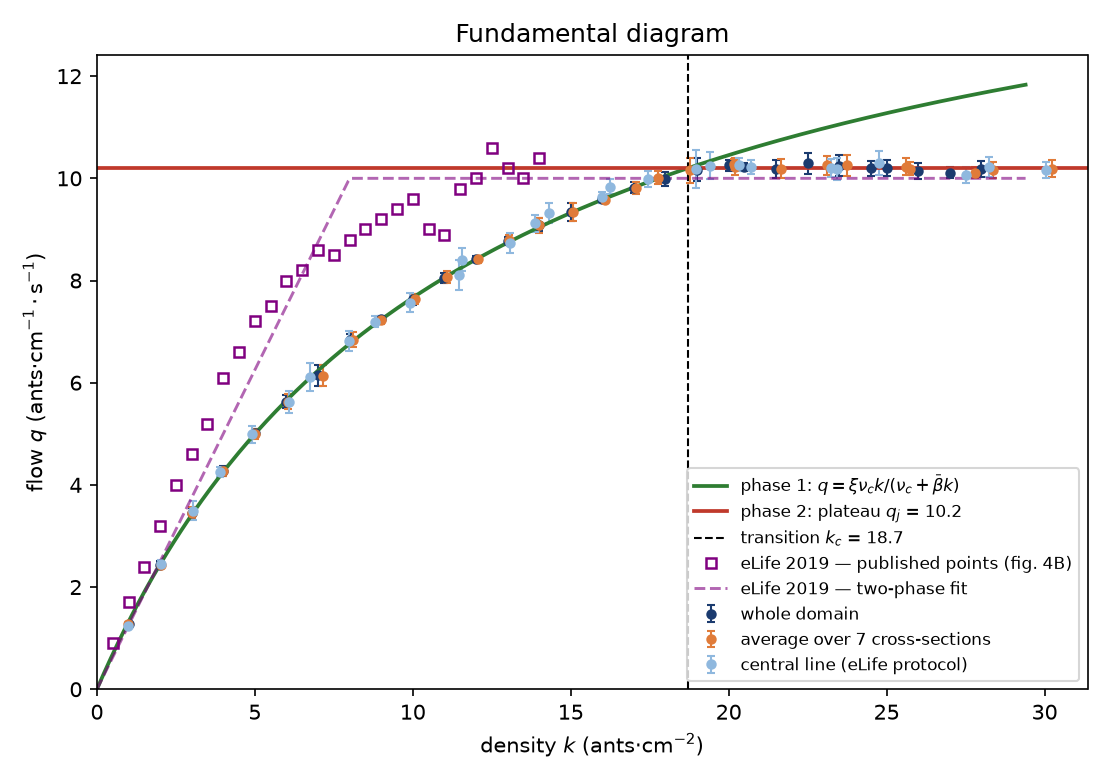
\includegraphics[width=0.78\linewidth]{diagramme_fondamental.png}
\caption{Fundamental diagram. Purple squares: published points of the article
(fig.~4B); dashed line: their two-phase fit. The model reproduces the saturating
shape and the plateau level, but reaches it later: between $k=3$ and $k=16$ it
lies below the measurements.}
\end{figure}

\begin{figure}[ht]
\centering
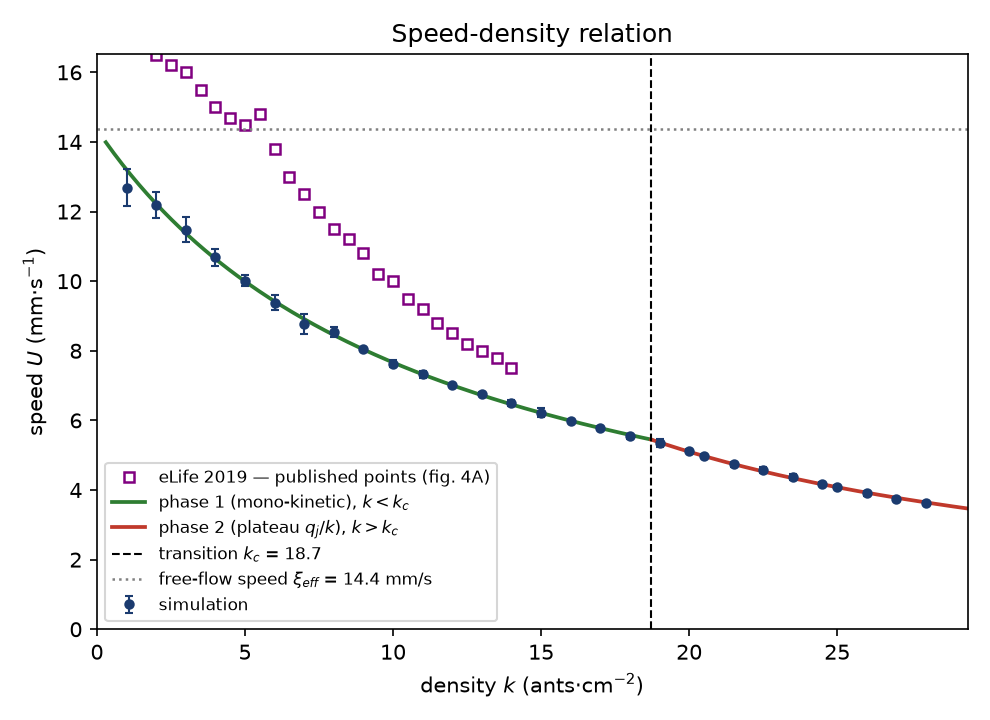
\includegraphics[width=0.72\linewidth]{vitesse_densite.png}
\caption{Speed--density relation. The offset is systematic: the published speed
starts at 17.5 mm/s and decreases slowly at first, whereas the model starts at
14.4 and decreases fastest at low density. The two curves meet around
$k\approx16$.}
\end{figure}

%======================================================================
\section{Departures from the reference model}\label{sec:gaps}

\begin{enumerate}\itemsep3pt
\item \textbf{Positional non-penetration removed} (user decision). The report
      enabled it ($g=1.0$, $\kappa=0.4$) and obtained $k_c\approx12.4$,
      $q_j\approx10.3$. Without it, overlap is no longer bounded, braking sees
      less physical density and saturates later. Measured cost: $k_c$ moves from
      $\sim12$ to $\sim19$.
\item \textbf{\code{standoff} wall law} instead of \code{tangential}
      (\S\ref{sec:wall}), with $c_{\rm wall}$ recalibrated from 10 to 2.
\item \textbf{Transverse remixing at periodic re-entry}, with its measured
      effect on the mixing observable.
\item \textbf{Deterministic tie-breaks} and a single random generator.
\item \textbf{$\xi$ lowered from 17 to 14}, \code{xi\_spread} kept at 0.2.
\end{enumerate}

The report's \emph{wall-escape} term (\code{use\_wall\_escape}) is implemented
but disabled; the \code{report} preset restores the report's wall law and
angular mode, but can no longer reproduce the published diagram exactly since
non-penetration has been removed.

%======================================================================
\section{Reference results}

Default configuration, 29 densities ($N=10$ to 280), 6 seeds, 40 s, 174 runs.

\begin{center}
\begin{tabular}{@{}lcc@{}}
\toprule
Quantity & Simulation & Reference \\
\midrule
Shape of the diagram & linear then \textbf{strict plateau} & two-phase \\
Phase-1 slope & 14.4 mm/s & $v_f\approx12$--21 \\
Effective braking $\bar\beta$ & 174 mm$^2$/s & 196 (measured on data) \\
Plateau $q_j$ & \textbf{10.21} & $\approx$ \textbf{10} \\
Transition $k_c$ & 18.6 & 8 (fit) / 10--12 (cloud) \\
Contacts ($k\leq20$) & $C=0.67\,k+0.54$ & $C=0.61\,k$ \\
Time cost $\Delta T$ & 0.15 s & 0.24 s \\
Segregation excess & $-0.03$ to $+0.09$ & --- \\
\quad without antennation & $+0.21$ to $+0.23$ & --- \\
\bottomrule
\end{tabular}
\end{center}

Across the 11 densities between $k=19$ and 28, the flow stays between 10.11 and
10.29: the plateau is \emph{strictly flat}, with no decline whatsoever, up to
one and a half times the maximum experimental density. The stopped fraction
there rises from 3 to 12\,\%: the flow slows down a great deal but does not
clog.

%======================================================================
\section{Limitations and open points}

\textbf{The knee does not move.} None of the magnitudes or rates tested
($k_\obj$, $c_{\rm avoid}$, $c_{\rm repulse}$, $c_\brake$, $\nu_\cruise$,
\code{xi\_spread}, $\sigma_\theta$) brings $k_c$ near 8: it stays between 13 and
19. The diagnosis lies in the speed \emph{at} the transition,
$U(k_c)=10q_j/k_c$: the two-phase description requires 12.5 mm/s, i.e.\ the
free-flow speed --- hence no slowdown at all before the knee --- whereas the
model gives 4 to 6. Structurally, $q(8)=10$ with $\xi=12.5$ requires
$\bar\beta\to0$. Increasing $c_\brake$ does bring $k_c$ closer to 8 but lowers
the plateau in the same proportion: the two are tied by the same constant.

\emph{But that knee does not exist in the data}: the published points start
bending at $k\approx3$ and saturate gradually (\S\ref{sec:elife}). ``$k_j=8$''
is a parameter of the two-phase fit, not a measurement, and Underwood describes
the cloud just as well. \textbf{The knee question is therefore largely a false
problem}: the model has the right qualitative \emph{shape}. What remains to be
explained is not the absence of a knee, but the fact that saturation arrives too
late --- a direct consequence of the next point.

\textbf{Speed is too low at intermediate densities.} The comparison with the
published points (\S\ref{sec:elife}) is unambiguous:

\begin{center}
\begin{tabular}{@{}lcccc@{}}
\toprule
$k$ (ants/cm$^2$) & 1 & 5 & 10 & 14 \\
\midrule
published $U$ (mm/s) & 17.2 & 14.5 & 10.0 & 7.5 \\
model $U$ (mm/s) & 12.7 & 10.7 & 7.6 & 6.7 \\
\bottomrule
\end{tabular}
\end{center}

Two components, of different natures.

\emph{A scale offset.} The published speed extrapolated to $k\to0$ is
$\sim$17.5 mm/s, which supports $\xi\approx17$ --- the model's original value,
not the 12.5--13 given by the braking profile measured on the trajectories we
hold. \textbf{The two data sources disagree by a factor $\sim$1.4 on speed}, and
this has not been resolved: the three available recordings (colonies 800, 3200,
12800) give a mean scalar speed of 10--12 mm/s where the published curve, which
aggregates 170 experiments, gives 15--17. Before recalibrating $\xi$, the origin
of that gap must be understood (trajectory smoothing protocol, inclusion or
exclusion of stopped ants, different sets of experiments).

\emph{A shape mismatch.} The published speed is nearly \emph{flat} up to
$k\approx3$ and then decreases, i.e.\ sigmoidal; the Monod law, by contrast,
decreases fastest at zero density. This means the real braking is
\textbf{weaker than linear at low density and stronger at high density}. That is
a structural constraint on the braking kernel which neither $\xi$ nor
$\bar\beta$ can satisfy, and it echoes the finding on the knee: it is not a
tuning problem.

\textbf{No stopped ants.} The data contain \textbf{4.7\,\%} of speeds below
1 mm/s --- the spike at zero in the histogram --- against 0.1\,\% in the model at
comparable density. This is the sharpest remaining gap, and precisely the
mechanism on which Dobramysl et al.\ (2024) base their explanation of the
plateau. First candidate for an extension.

\textbf{Uncalibrated lengths.} The measured braking range is $\sim5$ mm against
3 in the model, and the wall standoff distance suggested by the transverse
profiles is 2.5--4 mm against 1. Lengths were frozen by decision; they are the
next batch to calibrate, and the speed profile as a function of distance to the
frontal neighbour (\S\ref{sec:xi}) provides a direct method.

\textbf{Antennation without an explicit time cost.} The emergent $\Delta T$
(0.15 s) is of the right order but below the measured 0.24 s. A per-agent
antennation timer remains the natural extension (item B.1 of the project
backlog).

\textbf{Not tested.} Widths 5/10/20 mm, asymmetric foraging/returning
composition, bottleneck geometries, priority rules.

\end{document}
